%CPU y GPU -> femeninos
%Schedule -> planificación

%----------------------------------------------------------------------
%RESUMEN
El objetivo de este capítulo es introducir los conceptos de: 1) sistemas en tiempo real; 2) tipos de ejecución de tareas; 3) el algoritmo por defecto de los sistemas en tiempo real 4) sistemas embebidos heterogéneos; 5) arquitecturas de hardware y software de tarjetas gráficas; y 6) cómputo de propósito general en en unidades de procesamiento de gráficos.
%----------------------------------------------------------------------
%SISTEMAS EN TIEMPO REAL
\section{Sistemas en tiempo real}\label{sec:sistr}

Los sistemas en tiempo real son sistemas de cómputo cuyas tareas deben actuar dentro de limitaciones de tiempo precisas ante eventos en su entorno. Por lo que el comportamiento del sistema depende, no solo del resultado del cálculo, sino también del momento (tiempo) en que se produce \cite{Buta2011}.

\subsection{Tipos de ejecución de tareas}

Existen dos tipo de ejecución de tareas, las \textit{\textbf{preemptive}}, donde es necesario interrumpir temporalmente una tarea que está realizando un sistema de cómputo, para darle la oportunidad a otra con mayor prioridad, con el compromiso de reanudar la rezagada más adelante, y las \textit{\textbf{non-preemptive}} donde se requiere que termine la tarea actual para que posteriormente inicie una con mayor prioridad.

\subsection{Algoritmos de planificación}

Earliest Deadline First (EDF) es un algoritmo óptimo de planificación para sistemas de tiempo real, y acepta tareas en modo preemptive. Es un algoritmo muy extendido en sistemas en tiempo real debido a su optimalidad teórica en el campo no-preemptive, pero al momento de implementarlo en un planificador preemptive, el resultado puede acarrear un exceso de ejecución si se toma el peor caso \cite{EmbSysDes}. Por ello es necesario buscar alternativas de algoritmos que tengan un mejor desempeño en tareas específicas.

%----------------------------------------------------------------------
%GPU
\section{CPU}
La unidad de procesamiento central o CPU es un procesador de propósito general, lo que significa que puede hacer una variedad de cálculos, pero esta diseñado para realizar el procesamiento de información en serie, consta de pocos núcleos de propósito general. Aunque se pueden utilizar bibliotecas para realizar concurrencia y paralelismo, el hardware \textit{per se} no tiene esa implementación.

\section{GPU}
La unidad de procesamiento gráfico o GPU es un procesador especializado para tareas que requieren de un alto grado de paralelismo. La tarjeta gráfica en su interior puede contener una cantidad de núcleos de un orden de cientos hasta miles de unidades que son más pequeñas y que por ende, individualmente realizan un menor número de operaciones. Esto hace que la GPU esté optimizada para procesar cantidades enormes de datos pero con programas más específicos\cite{gpgpu}. Lo más común al utilizar la aceleración por GPU es ejecutar una misma instrucción a múltiples datos para aprovechar su arquitectura.

\subsection{Manycore y Multicore}
Es necesario destacar que los \textit{manycore} y los \textit{multicore} son utilizados para etiquetar a los CPU y los GPU, pero entre ellos existen diferencias. 
Un core de CPU es relativamente más potente, está diseñado para realizar un control lógico muy complejo para buscar y optimizar la ejecución secuencial de programas.
\vspace{0.3cm}
En cambio un core de GPU es más ligero y está optimizado para realizar tareas de paralelismo de datos como un control lógico simple enfocándose en la tasa de transferencia (\textit{throughput}) de los programas paralelos.
\vspace{0.3cm}
Con aplicaciones computacionales intensivas, las secciones del programa a menudo muestran una gran cantidad de paralelismo de datos. Las GPU se usan para acelerar la ejecución de esta porción código. Cuando un componente de hardware que está físicamente separado de la CPU y se utiliza para acelerar secciones computacionalmente intensivas de una aplicación, se le denomina acelerador de hardware. Se puede decir que las GPU son el ejemplo más común de un acelerador de hardware.

\subsection{Arquitectura Pascal}

%
 
\subsubsection{Memoria unificada} 
 La memoria unificada proporciona un único espacio de direcciones virtuales para la memoria de la CPU y GPU, permitiendo la migración transparente de datos entre los espacios de direcciones virtuales completos tanto de la tarjeta gráfica como del procesador. Esto simplifica la programación en GPUs y su portabilidad ya que no es necesario el  preocuparse por administrar el intercambio de datos entre dos sistemas de memoria virtual diferentes\cite{WPNV}.
 
%Asignar memoria unificada es tan simple como reemplazar llamadas a malloc o cudaMalloc con llamadas a cudaMallocManaged\cite{}.
 
\subsubsection{Computación preemptive}
Permite que las tareas de cómputo se reemplacen con granularidad a nivel de instrucción, en lugar de bloque de subprocesos, evitando el funcionamiento prolongado de aplicaciones que monopolizan el sistema y no dejan ejecutar terceras tareas. Obteniendo así, que las tareas puedan ejecutarse todo el tiempo que requieran ya sea para procesar grandes volúmenes de datos o qué esperen a que ocurran varias condiciones, mientras otras aplicaciones son computadas concurrentemente\cite{WPNV}.

\subsubsection{Balanceo de carga dinámico}
En versiones anteriores de las tarjetas, la asignación de recursos en las colas de cálculos y de gráficos debía decidirse antes de la ejecución, por lo que, una vez que se lanzaba la tarea, no era posible reasignarla sobre la marcha. Un problema añadido que existía, era que si una de las colas se quedaba sin trabajo antes que la otra no podía iniciar un nuevo trabajo hasta que ambas colas terminen completamente\cite{PasAna}.
\vspace{0.3cm}
La arquitectura Pascal introdujo el soporte para balanceo de carga dinámico \cite{AnPasc},  ayudando a la aceleración del cómputo de tareas asíncronas.

\subsubsection{Operaciones atómicas} 
Las operaciones atómicas de memoria frecuentemente son importantes el cómputo de alto rendimiento ya que permiten que los hilos concurrentemente lean, escriban y modifiquen variables compartidas. La arquitectura Pascal nos permite realizar estas operaciones pero ahora con la ventaja de trabajar sobre memoria unificada.

\subsection{GPGPU}
El cómputo de propósito general en unidades de procesamiento de gráficos o GPGPU es utilizado para acelerar el procesamiento realizado tradicionalmente por la CPU únicamente, donde la GPU actúa como un coprocesador que puede aumentar la velocidad del trabajo \cite{GpuCpu}.

\begin{figure}[ht]
  \centering
    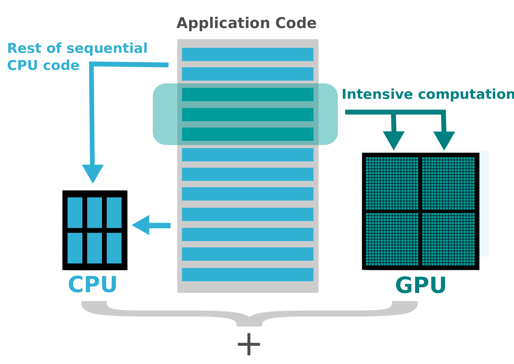
\includegraphics[scale=0.9]{img/gpgpu}
    \caption{Aceleración de programas en GPUs\cite{gpgpu}.}
    \label{fig:gpgpu}
\end{figure}

La unificación de los espacios de memoria facilita el GPGPU ya que no hay necesidad de transferencias explícitas de memoria entre el host y el dispositivo.


%----------------------------------------------------------------------
%SISTEMAS EMBEBIDOS
\section{Sistemas embebidos}

Un sistema embebido es un sistema de cómputo diseñado para realizar tareas dedicadas, donde el mayor retos es realizar tareas específicas donde la mayoría de ellas tengan requerimientos de tiempo real \cite{LimPree}.

\subsection{Sistemas embebidos heterogéneos}
%
\vspace{0.3cm}
En los últimos años los sistemas embebidos han ido demandando nuevas características debido a su rápida adopción en el mercado. Con lo que surge el desarrollo de sistemas embebidos heterogéneos, donde está contemplado realizar una gran cantidad de cómputo pero con una gran eficiencia tanto energética como en espacio.
\vspace{0.3cm}

Actualmente la empresa NVIDIA tiene en su catálogo sistemas embebidos heterogéneos con un gran soporte y bibliotecas para el cómputo de alto rendimiento. Dichos sistemas cuentan con la arquitectura pascal de última generación \cite{GPUArt}, la cual permite compartir memoria entre CPU y GPU.

\subsubsection{Jetson TX2}

% Framework
Debido a que la mayoría de las GPU en sistemas embebidos no son de naturaleza preemptive, es importante programar los recursos de GPU de manera eficiente en múltiples tareas \cite{TX2I} ya sea de planificación o memoria, lo que permite pensar en un framework que ayude a la administración de sus características. 

Las características del sistema:

\begin{table}[!tb]
  \begin{center}
        \scriptsize
    \begin{tabular}{|m{3.5cm}|m{4cm}|}
     \hline
    \cellcolor{lightgray} & \cellcolor{lightgray} \textbf{Descripción}\\ 
     \hline
     Arquitectura & NVIDIA Pascal GPU\\
     \hline
     CPU & 2 Denver 64-bit CPUs + Quad-Core A57 Complex\\
     \hline
     Memoria & 8 GB L128 bit DDR4 Memory\\
     
&32 GB eMMC 5.1 Flash Storage\\
     \hline
&Connectivity to 802.11ac Wi-Fi and Bluetooth-Enabled Devices\\
     \hline
&10/100/1000BASE-T Ethernet\\
     \hline
    \end{tabular}
    
    \caption{Especificaciones del sistema.}
    \label{tab:table1}
  \end{center}
\end{table}
aa

\section{Resumen}

%En este capítulo se presenta una breve introducción a la seguridad de la información, la importancia de incluirla en los sistemas de software y las amenazas a las que están expuestos los sistemas. Se hace un énfasis en la inclusión de la seguridad en la etapa de diseño de un sistema, donde se explica que utilizar guías para proporcionar un nivel de seguridad a un sistema en diseño disminuye las posibilidades de una amenaza al sistema ya implementado. 


